\let\negmedspace\undefined
\let\negthickspace\undefined
\documentclass[journal]{IEEEtran}
\usepackage[a5paper, margin=10mm, onecolumn]{geometry}
\usepackage{tfrupee}  % Include tfrupee package
\usepackage{gvv-book}
\usepackage{gvv}
\usepackage{cite}
\usepackage{amsmath, amssymb, amsfonts, amsthm}
\usepackage{algorithmic}
\usepackage{graphicx}
\usepackage{textcomp}
\usepackage{xcolor}
\usepackage{txfonts}
\usepackage{listings}
\usepackage{enumitem}
\usepackage{mathtools}
\usepackage{gensymb}
\usepackage{comment}
\usepackage[breaklinks=true]{hyperref}
\usepackage{tkz-euclide}
\usepackage{longtable}
\usepackage{multirow}
\usepackage{hhline}
\usepackage{lscape}
\usepackage{inputenc}  % Automatically handles various encodings

\setlength{\headheight}{1cm}  % Set header height
\setlength{\headsep}{0mm}     % Set header separation
\setlength{\intextsep}{10pt}  % Space between text and floats

\numberwithin{equation}{enumi}
\numberwithin{figure}{enumi}
\renewcommand{\thetable}{\theenumi}

\begin{document}

\bibliographystyle{IEEEtran}
\vspace{3cm}

\title{12.8.3.14}
\author{EE24BTECH11020 - Ellanti Rohith}
\maketitle

\renewcommand{\thefigure}{\theenumi}
\renewcommand{\thetable}{\theenumi}

\textbf{Question}: Using the method of integration find the area of region bounded by lines: $2x+y=4,3x-2y=6\text{ and } x-3y+5=0$.
\\
\vspace{3.5pt}


\textbf{Theoretical Solution:} \\
\textbf{By Integral:}\\
Let the three lines be defined as:  
\begin{enumerate}
    \item Line $ L_1: 2x + y = 4 $,  
    \item Line $ L_2: 3x - 2y = 6 $,  
    \item Line $ L_3: x - 3y + 5 = 0 $.  

\end{enumerate}
  
\subsection*{ $L_1: 2x + y = 4$ and $L_2: 3x - 2y = 6$}

\begin{align*}
\myvec{
2 & 1 & 4 \\
3 & -2 & 6
}
\xrightarrow{R_2 \to R_2 - \frac{3}{2}R_1}
\myvec{
2 & 1 & 4 \\
0 & -\frac{7}{2} & 0
}
\xrightarrow{R_1 \div 2, \, R_2 \div -\frac{7}{2}}
\myvec{
1 & \frac{1}{2} & 2 \\
0 & 1 & 0
}
\xrightarrow{R_1 \to R_1 - \frac{1}{2}R_2}
\myvec{
1 & 0 & 2 \\
0 & 1 & 0
}
\end{align*}

Solution: $x = 2, \, y = 0$.

\subsection*{$L_2: 3x - 2y = 6$ and $L_3: x - 3y = -5$}

\begin{align*}
\myvec{
3 & -2 & 6 \\
1 & -3 & -5
}
\xrightarrow{R_2 \to R_2 - \frac{1}{3}R_1}
\myvec{
3 & -2 & 6 \\
0 & -\frac{7}{3} & -7
}
\xrightarrow{R_1 \div 3, \, R_2 \div -\frac{7}{3}}
\myvec{
1 & -\frac{2}{3} & 2 \\
0 & 1 & 3
}
\xrightarrow{R_1 \to R_1 + \frac{2}{3}R_2}
\myvec{
1 & 0 & 4 \\
0 & 1 & 3
}
\end{align*}

Solution: $x = 4, \, y = 3$.

\subsection*{ $L_1: 2x + y = 4$ and $L_3: x - 3y = -5$}

\begin{align*}
\myvec{
2 & 1 & 4 \\
1 & -3 & -5
}
\xrightarrow{R_2 \to R_2 - \frac{1}{2}R_1}
\myvec{
2 & 1 & 4 \\
0 & -\frac{7}{2} & -7
}
\xrightarrow{R_1 \div 2, \, R_2 \div -\frac{7}{2}}
\myvec{
1 & \frac{1}{2} & 2 \\
0 & 1 & 2
}
\xrightarrow{R_1 \to R_1 - \frac{1}{2}R_2}
\myvec{
1 & 0 & 1 \\
0 & 1 & 2
}
\end{align*}


Solution: $x = 1, \, y = 2$.
The required area is the sum of:  
\begin{enumerate}
    \item The area bounded by $ L_1 $ and $ L_3 $ over the interval $ x = 1 $ to $ x = 2 $, and  
    \item The area bounded by $ L_2 $ and $ L_3 $ over the interval $ x = 2 $ to $ x = 4 $.  
\end{enumerate}

The required area can be calculated as the integral of the difference of the functions:  



\begin{align}
f(x) = 
\begin{cases} 
     \dfrac{7}{3}x - \dfrac{7}{3}
 & \text{for } 1 \leq x \leq 2, \\[10pt]
 -\dfrac{3x}{2} + \dfrac{14}{3}, & \text{for } 2 < x \leq 4.
\end{cases}
\end{align}



The area is given by:  
\begin{align}
   \text{Area} = \int_{1}^{2} \left( \frac{7}{3}x - \frac{7}{3} \right) \, dx
+ \int_{2}^{4} \left( -\frac{3x}{2} + \frac{14}{3} \right) \, dx
\end{align}
Thus, the total area is:  
\begin{align}
   \text{Area} = \frac{7}{6} + \frac{1}{3} = \frac{9}{6} = \frac{3}{2}. 
\end{align}

$\text{ Area }= \dfrac{3}{2} \text{ square units.}$\\
\textbf{Simulation}:
\\
Splitting the intervals  with step size $h = 0.01$
\\
\textbf{Trapezoidal Rule:}\\
Summing area of  all Trapezoids to give area under a given curve $f(x)$\\
\begin{align}
	A &\approx \frac{h}{2} \brak{(f(x_{0}) + f(x_{1})) + (f(x_{1}) + f(x_{2})) + \dots + (f(x_{n-1}) + f(x_{n}))} \\
	A &\approx \frac{h}{2} \brak{f(x_{0}) + 2 \sum_{i=1}^{n-1} f(x_{i}) + f(x_{n}) }\\
    A_{n+1} &= A_{n} + \frac{h}{2} \brak{y_{n} + y_{n+1}}
    \end{align}
    \begin{align}
    \text{This is the required difference equation:}\\
x_{n+1} &=x_{n}+h\\
y_{n+1} &=y_{n}+hy'_{n}\\
A_{n+1} &= A_{n} + \frac{h}{2} \brak{2y_{n} +  h y^{\prime}_{n}}\\
y'_{n}&=\begin{cases} 
     \dfrac{7}{3}
 & \text{for } 1 \leq x_{n} \leq 2, \\[10pt]
 -\dfrac{3}{2} , & \text{for } 2 < x_{n} \leq 4.
\end{cases}
\end{align}
By simulation, the answer turns out to be $1.49933450000053  \approx \dfrac{3}{2}.$

\begin{figure}[h!]
    \centering
    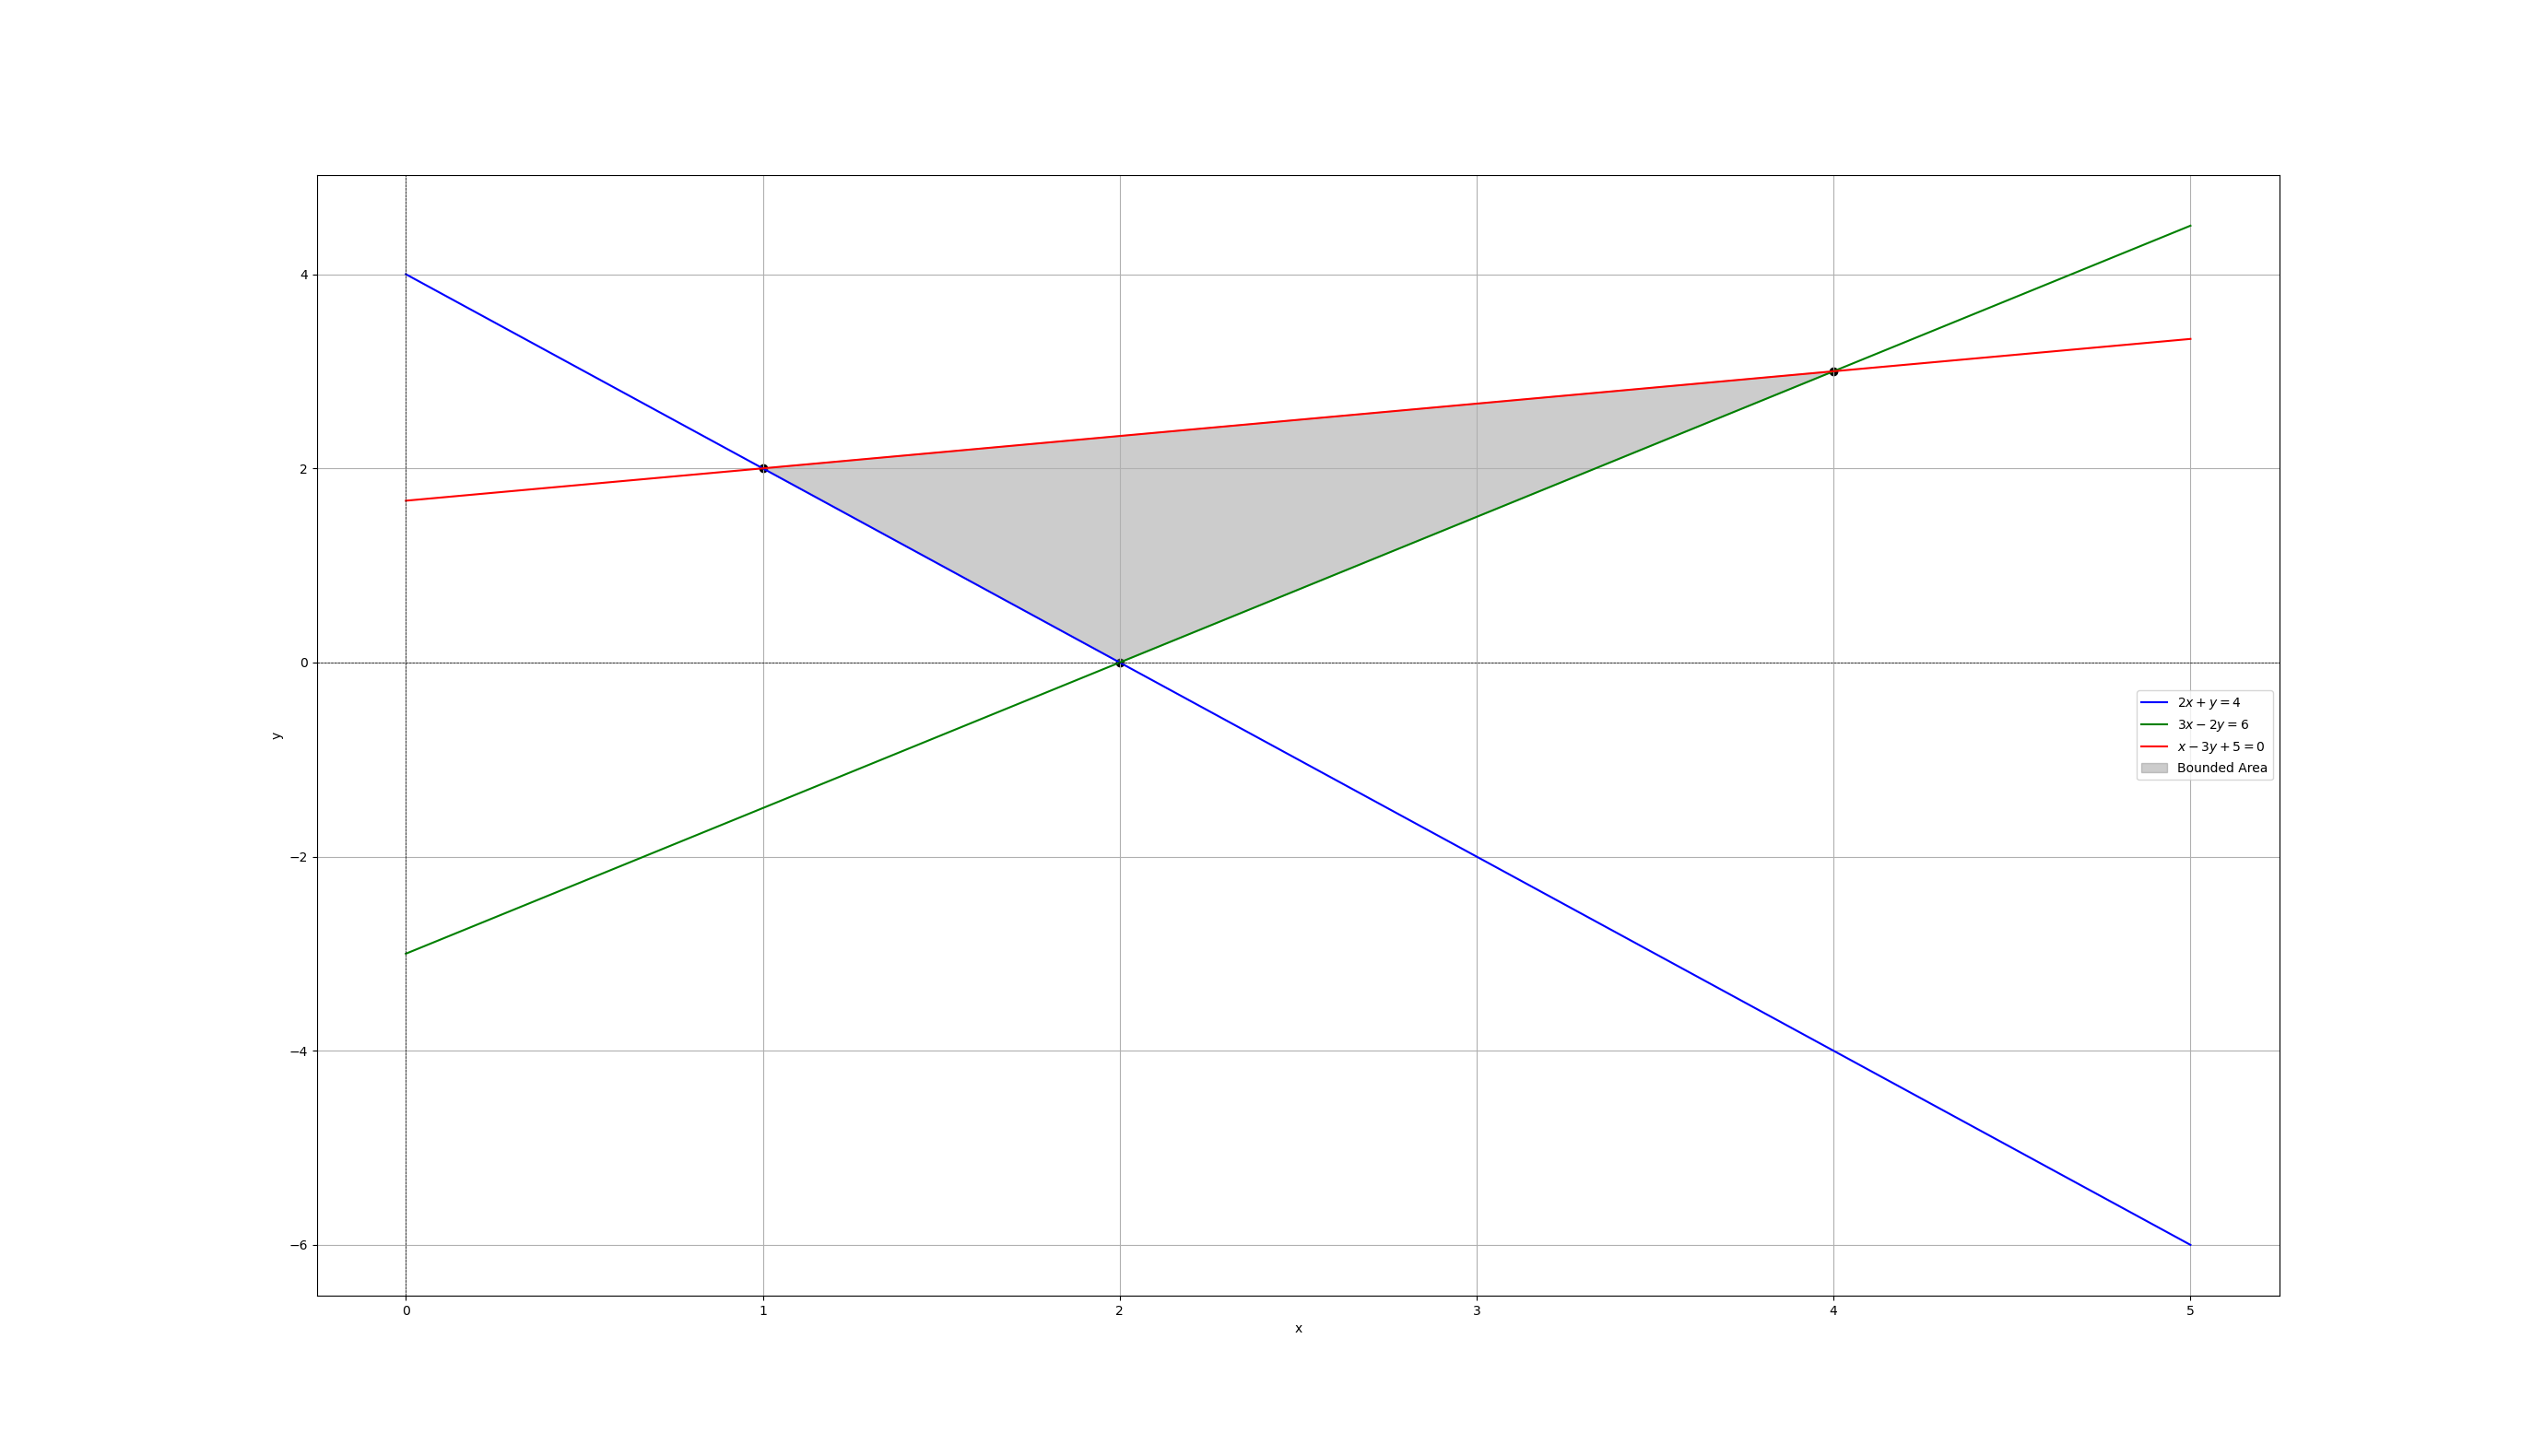
\includegraphics[width=\columnwidth]{Figs/Figure_1.png}
    \caption{Plot of three lines and the bounded area.}
\end{figure}

\end{document}

